% !TeX root = ../../thesis.tex
\chapter{Introduction} \label{ch_introduction}

% Some dummy code to get at least 1 entry in the nomenclature.
\nomenclature{$\Theta$}{A nice symbol}
% Some dummy code to get at least 1 entry in the list of
% abbreviations.
\newglossaryentry{md}{name={MD},description={molecular dynamics}}

\section{General introduction}
Crystallographic texture has a marked influence on the properties of polycrystalline coatings. Seemingly unrelated parameters (properties) such as corrosion resistance, hardness, magnetic properties, porosity, and contact resistance are all texture dependent~\cite{Schlesinger2010}. Some properties such as macroscopic magnetic anisotropy do not even exist if the sample is not textured~\cite{Dinnebier2008}.

Every deposition method has its specific parameters used to control the process. These are used to optimize the resulting textures, but the relation to the fundamental texture-forming quantities (i.e. the local conditions on the deposited material surface) is usually missing. The problem is that they are inaccessible after the deposition and it is not clear how they could be measured during the deposition. 

Irrespective of which type of deposition technique is used, texture formation is controlled by interfacial energy, surface diffusivity of adatoms, grain boundary mobility and grain boundary and lattice diffusion~\cite{Szpunar1997, Suwas2014}. These properties together then affect the fundamental processes: nucleation, crystal growth and grain boundary motion~\cite{Barna1998}. Understanding how the texture in films is formed and how it can be controlled during the deposition process, is beneficial for the development of methods of texture optimization~\cite{Szpunar1997}. 

The anisotropy in crystal growth in general must originate from the anisotropy on the interfaces of the growing crystal with its surroundings - the substrate and the parent phase. In electrodeposition, the surface conditions may dynamically change due to local concentration evolution of the many present thermodynamic species in the solutions and their interactions with the deposit surface. 

In such situations, mathematical models of the process are useful to suggest some interpretation to the observed behaviors to gain better insight. This thesis elaborates on the possible impact of anisotropy in interface energy on the orientation selection during repeated nucleation on the course of the film growth. 

Of the deposition methods, the electrodeposition is particularly interesting, because
\begin{itemize}
	\item the (anisotropic) surface conditions are highly adjustable by additives and deposition conditions,
	\item the current or voltage transients provide valuable integral feedback on the surface processes in-situ, so there is more information available than in other methods,
	%	\item it can be carried out in a highly localized way (e.g. during electrochemical scanning microscopy), which allows higher control ???!,
	%	\item the direction of the deposition reaction is controlled by the sign of applied voltage, which allows pulsed regime, where deposition and stripping are repeated in rather short cycles. This adds completely new dynamics to the deposition process and provides additional perspective to tune the deposit properties, 
	\item it is industrially relevant.
\end{itemize}
For these reasons, this thesis focuses more on electrodeposition than on other deposition methods. However, the interface energy is relevant for all the others as well, hence the implications of its anisotropy are in principle applicable to any other deposition method. 

Electrodeposition is a highly industrially relevant process used for many applications like metal deposition for the fabrication of integrated circuits, deposition for magnetic recording devices (heads, disks), and deposition
of multilayer structures~\cite{Schlesinger2006}, to name a few. Similarly like in other methods, the electrodeposits are usually polycrystalline and exhibit pronounced crystallographic texture, which is affected by many factors. 


%This highlights the utility of simulation tools, which allow to set the anisotropy in interface energy and kinetic coefficient independently, because in practice the individual effects may be hard or impossible to distinguish. Among such tools is (multi-)phase field method.

The interface energy is particularly important for the nucleation, which is in turn the main process of how grains with new orientations are introduced during the film growth. To the best of author's knowledge, the relation between the interface energy anisotropy and the anisotropy in nucleation barrier as function of local crystallographic orientation has not been fundamentally investigated. This work intends to bring more insight into this relation using different simulation approaches.

%The following sections provide some fundamental information about the deposition process and as-deposited mictrostructures - Structure-Zone model, Winand diagrams and how the calssical nucleation theory is modified by the presence of anisotropy in interface energy.


\section{Goals of the thesis}

\noindent\fbox{%
	\parbox{\textwidth}{%
		There are two main goal of this thesis:
		\begin{enumerate}
			\item Develop a methodology based on the multi-phase-field model~\cite{Moelans2008} capable of determining the nucleation barrier anisotropy 
			\item Bring insight into the role of anisotropy in interface energy for nucleation during polycrystalline film growth and the possible impact on texture evolution.			
		\end{enumerate}
	}%
}


The following \textbf{key objectives (KO)} were set to accomplish the main goals:
\begin{description}
	\item[KO1] To develop and benchmark the multi-phase field model~\cite{Moelans2008} including the anisotropic interface energy.
	\begin{description}
%		\item[KO1.1] Implement the multi-phase field model~\cite{Moelans2008} with inclination-dependent interface energy and validate the implementation
		\item[KO1.1] Derive the governing equations for all the compared model variants.
		\item[KO1.2] Define quantitative benchmark problems to validate both the implementation and the model variants in terms of the anisotropic curvature driving force.
		\item[KO1.3] Implement own numerical solver.
		\item[KO1.4] Compare the model variants and draw conclusions.
	\end{description}
\end{description}
\noindent\textbf{Comment:} there exist multiple variants of the model~\cite{Moelans2008}, but not all of them were used with inclination-dependent interface energy, hence the governing equations for these must be derived. Additionally, no systematic comparison was made, hence it was not obvious which model variant would be suited the best for the current application.

\begin{description}
	\item[KO2] Develop a methodology based on the multi-phase-field model~\cite{Moelans2008} capable of determining the nucleation barrier anisotropy.
	\begin{description}
		\item[KO2.1] Work out the concept of the whole methodology. Specify the requirements on the model, the simulation geometry and if necessary carry extend the model further.
		\item[KO2.2] Implement the model and validate its key aspects 
		\item[KO2.3] Validate the methodology on some problem with known solution.
		\item[KO2.4] Demonstrate usability of the developed methodology on a problem without known solution.
	\end{description}
	\item[KO3] Determine how anisotropy of the nucleation barrier (different for differently oriented nuclei) relates to interface energy anisotropy and local crystallography
	\begin{description}
		\item[KO3.1] Analyze and specify the problem
		\item[KO3.2] Implement a solver which is able to return the nucleation barrier for each pair of the substrate and particle orientations
		\item[KO3.3] Using the solver investigate how the nucleation barrier depends on the orientations
	\end{description}
	\item[KO4] Demonstrate in a 2D Monte Carlo simulation of growing polycrystalline film how such anisotropy in nucleation barrier may affect texture evolution
	\begin{description}
		\item[KO4.1] Develop an orientation-sampling algorithm based on the anisotropic nucleation probability
		\item[KO4.2] Develop and validate the 2D Monte Carlo simulation algorithm incorporating nucleation with the orientation sampling
		\item[KO4.3] Carry out a parameter study to showcase the impact of nucleation with isotropic or anisotropic interface energy on texture evolution under different conditions
	\end{description}
	\item[KO5] Apply the novel theoretical insights to some real-world practical system
	\item[KO6] Synthesize the findings and propose future directions of the research
\end{description}

%The development of methodology to determine anisotropy of nucleation barrier based on phase-field method (KO1.2) is challenging and required further breakdown of this Key Objective. For better comprehensibility, these were listed separately
%
%\begin{description}
%	\item[KO1.2] Develop methodology based on phase-field method
%	\begin{description}
%		\item[KO1.2.1] Propose the methodology and review phase-field method
%		\item[KO1.2.2] Specify requirements on the model and simulated system geometry
%		\item[KO1.2.3] Work out the necessary extensions of an existing phase field model including anisotropy of interface energy and kinetic coefficient
%		\item[KO1.2.4] Implement the phase field model 
%		\item[KO1.2.5] Develop well defined benchmark problems to validate the implementation
%		\item[KO1.2.6] Demonstrate usability of the developed methodology
%	\end{description}
%\end{description}

%This thesis explores the effect of anisotropic interface energy on nucleation and growth of polycrystalline deposits in various simulation concepts. It is known that the anisotropy in interface energy affects the equilibrium stable shape of a particle (on a plane). Also, it is known that the nucleation probability is proportional to the particle area (in 3d to its volume).


%The anisotropic nature of monocrystals implies anisotropy of the interfaces they have with their surroundings. This translates into anisotropy of both thermodynamic and kinetic properties which are tied with the interface, especially the specific interface energy and the kinetic coefficient of the deposition/dissolution reaction. Even though it is natural to expect that both are manifestations of a single surface condition, because both quantities are used 

\section{Thesis overview} \label{sec_Thesis_overview}
This thesis explores how anisotropy in surface energy affects the course of crystallographic texture evolution in polycrystalline coatings, with emphasis on orientation selection in repeated nucleation seen within the framework of classical nucleation theory. 

%In order to bring insight in this matter, the problem was first analyzed (KO1.1) \colorbox{red}{IN CHAPTER} and two different approaches to determine anisotropy in interface energy were developed (KO1.2 and KO1.3). 

The Chapters~\ref{ch_anisoIEintro} and~\ref{ch_introPF} provide the necessary fundamentals and relevant literature review. The subsequent chapters contain the original research carried out by the author.

%The Chapters~\ref{ch_paper1} and~\ref{ch_paper2} contain the results published as~\cite{Minar2022} and~\cite{Minar2024}, respectively. The Chapter~\ref{ch_NPA_PF_methodology} contains unpublished results on the phase-field methodology to obtain so-called shape factor of a heterogeneous nucleus. The shape factor can be related to the nucleation probability for the particular shape.

The Chapter~\ref{ch_anisoIEintro} provides fundamentals related to the surface energy, like the capillary vector formalism used to describe its anisotropy, interface stiffness, the Wulff shapes, the force balance in triple junctions and Winterbottom construction to obtain equilibrium stable shapes on a plane. Fundamentals of classical nucleation theory are provided as well.

The Chapter~\ref{ch_introPF} introduces the phase-field method. In a step-wise manner, the fundamentals of the method are covered. First, the Allen-Cahn equation is described, which represents phase evolution under the effect of isotropic curvature driving force. Then, the standard ways of adding a) anisotropy in interface energy, b) multiple phase-fields in the simulation domain (and both) are reviewed. Challenges and limitations of the various phase-field models are discussed. Also, a section was included, commenting on the importance of benchmarking the performance of applied multi-physics phase-field models and the current practice of their usage and presentation within the scientific community.

In the Chapter~\ref{ch_paper1}, there is a comprehensive description of an existing multi-phase field model and how and why it was extended. Three different variants of the same model were obtained. Two different benchmark problems to quantitatively test how the models reproduced the anisotropic curvature driving force were developed. A thorough parameter study was conducted to provide exhausting information on the model behavior in different settings. Only in a third benchmark problem involving triple junctions showed, that there was in fact a significant difference in the behavior of the model variants. Results in this chapter were published in~\cite{Minar2022}. The Key Objective KO1 and all its sub-objectives are fulfilled in this chapter.

The Chapter~\ref{ch_NPA_PF_methodology} presents the \textit{domain scaling} methodology, which was developed to determine so-called shape factor of a heterogeneous nucleus. That quantity is closely tied with nucleation barrier and thus the nucleation probability. The multi-phase field model was used to obtain the equilibrium stable shape of nucleus needed for \textit{domain scaling} to work. Because the model extensions carried out in Chapter~\ref{ch_paper1} were still not sufficient to realize the developed methodology, additional extensions were introduced, building on top of the knowledge and implementation in Chapter~\ref{ch_paper1}. The methodology was validated and showcased on an example of a nucleus on top of a grain boundary within a substrate, which is a case where the shape does not have analytic solution. The Key Objective KO2 and all its sub-objectives are resolved in this chapter.

Then follows the Chapter~\ref{ch_paper2}, which employs the so-called Winterbottom construction to obtain the equilibrium stable shape of the nucleus. Because this method is very computationally efficient, the nucleation barrier as function of the substrate and nucleus orientation could be determined with great resolution. The obtained \textit{shape-factor-orientation maps} are a visualization of the nucleation barrier orientation dependence (orientation of both the substrate and nucleus with anisotropic interface energy). These were then used as an input to a custom orientation-sampling algorithm for the nuclei. Using this, the orientation of nuclei introduced during a Monte Carlo simulation of 2D polycrystalline film growth was determined. A parametric study was conducted to identify the impact of the anisotropy in interface energy on the texture evolution, when compared to the isotropic interface energy. The obtained insights were used to qualitatively explain an abrupt change in texture which observed in electrodeposited nickel~\cite{Alimadadi2016}. Results in this chapter were published in~\cite{Minar2024}. The Key objectives KO3, KO4 and KO5 are accomplished in this chapter

The Chapter~\ref{ch_conclusion} summarizes the work and its main contributions and proposes directions for future research, which fulfills the Key Objective KO6.

A number of appendices was included in the work to provide relevant information, which was not essential for understanding the results in the main text. These were mostly used for mathematical derivations, details on implementation of numerical methods or other supplementary information improving transparency and reproducibility of this research. In order to achieve even higher reproducibility, all the source MATLAB code used to deliver the results in the published works was made available in online repositories~\cite{Minar2022dataset} and~\cite{Minar2023dataset} together with usage instructions.

\section{Microstructure formation in coatings}
This section contains review of literature related to formation of textures in polycrystalline coatings with emphasis on the underlying processes which are common to all the deposition methods, like electrodeposition, physical vapor deposition or sputtering. 

Microstructure here denotes both the morphology on the surface, shape and size of grains and their crystallographic texture.

The experimental investigations of the texture-forming factors in deposits are usually specific for the particular deposition method, like physical vapour deposition (PVD), sputtering or electrodeposition. Despite some obvious differences between the methods, it is natural to expect the textures to be formed by the same mechanisms. These are necessarily altered by the method-specific deposition conditions, thus giving rise to some behaviors which are then considered as standard for that type of deposition. 

For example, the Structure Zone Model (SZM)~\cite{Barna1998, Anders2010} is often used to describe the dependence of microstructure on the relative deposition temperature in PVD and sputtering methods. The Structure-zone model was extended several times to new parameter regions, for an example of a rather recent model see Figure~\ref{fig_SZM_and_Winand}b. On the other hand, in the electrodeposition rather the Winand diagram~\cite{Winand1992} is used instead, having the axes representing degree of chemical surface inhibition and current density, i.e. deposition rate (see Figure~\ref{fig_SZM_and_Winand}a). Both of these can be perceived as state diagrams, where the individual regions qualitatively indicate the one microstructure/morphology which is most likely to be stable for those deposition conditions. Interestingly, in electrodeposition the crystallographic texture of the coating does not necessarily imply a particular deposit morphology~\cite{Winand1992}.

\begin{figure}
	\centering
	\begin{tikzpicture}
		\draw (0,0) node [above left, inner sep =0] {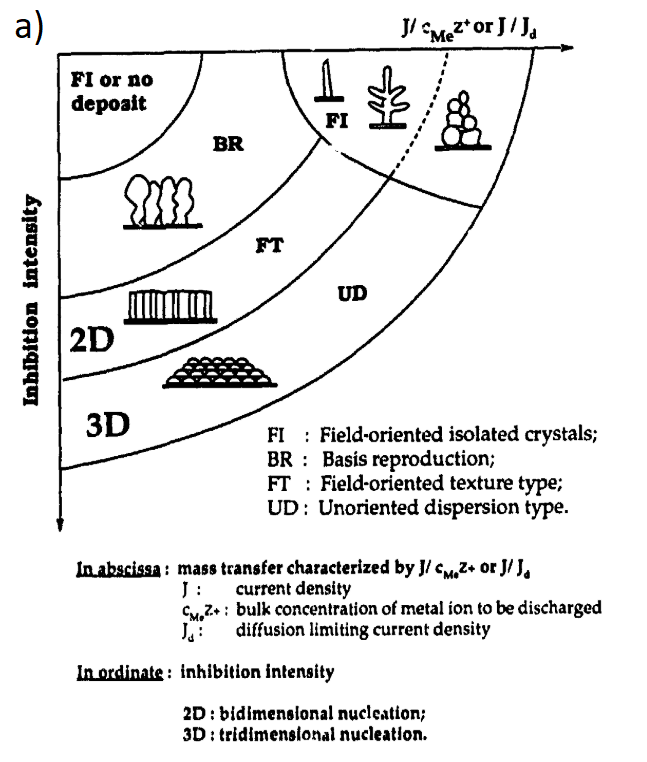
\includegraphics[width=0.55\textwidth]{Winand1992_diagram.png}};
		\draw (0,0) node [below left, inner sep =0] {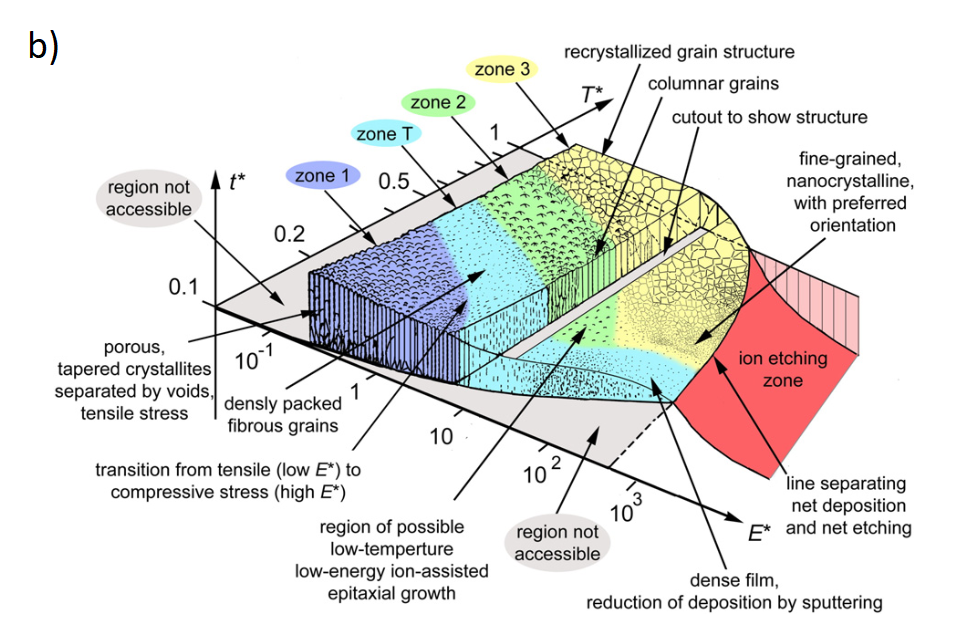
\includegraphics[width=0.7\textwidth]{Anders2009_SZM_.png}};
	\end{tikzpicture}
	\caption[Examples of Structure Zone Model and Winand diagram]{Simplified empirical diagrams, in a) Winand diagram for electrodeposition~\cite{Winand1992}, in b) Structure-zone model for high-energy deposition from vapor~\cite{Anders2010}.}
	\label{fig_SZM_and_Winand}
\end{figure}

Barna~\cite{Barna1998} claims, that the different crystallographic textures observed in PVD or sputter deposition can be correlated to the respective \textit{structure zone}. Specifically, he uses the terms \textit{competitive growth texture} and \textit{restructuration growth texture}, which correspond to the ones where the resulting texture depends on either the anisotropy in growth rate or on the concurrent minimization of surface and grain boundary energy, respectively.

In electrodeposition, the situation is more complicated than in PVD or sputtering by the presence of the double layer on the metal surface and the complex interplay of the electric field and chemical reactions between all the species.  Nevertheless, experimental work largely shows that, as far as three-dimensional nucleation is concerned, the same observations are made in electrocrystallization
and in physical crystallization~\cite{Winand1992}: increasing the deposition rate and/or increasing the inhibition usually results in increased nucleation rate and thus eventually in the reduction in the deposit grain size.

The inhibition refers to some specific interactions between the deposit and the parent phase. The inhibiting species attaches to low-energy sites where the growth might easily proceed and then the adatoms must find another spot to settle down, having their lifetime before being incorporated into the crystal potentially prolonged and thus increasing the nucleation probability~\cite{Winand1992}. The inhibitor may be a natural constituent of the electrolyte in electrodeposition or simply some impurity. In PVD deposition of Al with variable amounts of oxygen, it was observed that increased oxygen amounts reduced the grain size up to nanocrystalline or even amorphous coating of alumina~\cite{Barna1998}.

A separate field of research involves stress in the deposits~\cite{Thornton1989, Thompson1993, Chason2015, Abadias2018}. Both tensile and compressive stress are observed in the deposits depending on the deposition conditions and deposited material. Generally speaking, higher temperatures and lower deposition rates (i.e. deposition closer to thermodynamic equilibrium) lead to behavior, where a compressive stress develops with increasing thickness of the film, but after the deposition stops, the stress either completely or partly relaxes. This is highly dependent on the material too, where materials with higher self-diffusion coefficient (lower melting point) tend to exhibit such behavior~\cite{Chason2002}. On the other hand, high growth rates and low deposition temperatures (i.e. rather off-equilibrium deposition) lead to tensile stresses, which do not relax after the deposition termination. Materials with lower self-diffusion coefficients (higher melting points) are associated with these. Another source of stress can be interactions with the substrate.

Stress can suppress or promote grain growth~\cite{Thompson1993}. It is then natural to consider stress relaxation as another texture-forming process. As was mentioned in the Introduction, the fundamental texture-forming quantities are interfacial energy, surface diffusivity of adatoms, grain boundary mobility and grain boundary and lattice diffusion~\cite{Szpunar1997, Suwas2014}. However, it is the particular state of the material and the deposition conditions, which then drives the deposit to evolve in particular ways.

Thompson~\cite{Thompson1993} developed an abstracted model of columnar microstructure and expressed its total strain and total interface energy as function of thickness. Because the thickness dependence of these energies was different, the model suggested that the texture could be dominated by minimization of interface energy below certain (temperature-dependent) thickness and above it, the texture would be dominated by the strain energy minimization. Especially in the light of the previous paragraph, it is clear that the stress state of a real deposit does not depend only on the deposit thickness. Nevertheless, the idea of having different mechanisms competing over the course of texture/morphology evolution as the film thickness increases is strongly based in experimental observation. Also, the terms \textit{interface-energy minimization texture} or \textit{strain-energy minimization texture} are used in practice~\cite{Alimadadi2016}.

Specifically in electrodeposition, the inhibition in relation to the morphology and texture was studied extensively~\cite{Winand1992}. Amblard~\cite{Amblard1979} determined the particular species responsible for the texture variation in nickel electrodeposits from Watts electrolyte when varying the pH, current density and adding separately a brightening and leveling agents. These species selectively inhibited the metal surface and thus introduced different textures. A more recent study~\cite{BergenstofNielsen1997} reviewed other hypotheses about the possible texture-forming processes in nickel electrodeposition from Watts electrolyte and after transmission electron microscopy study of one deposit, they concluded that the inhibition was the most likely scenario. 

The same group later proposed~\cite{Rasmussen2001}, that the texture of an electrodeposit could develop from a zone mainly affected by the substrate (epitaxy, chemical reactions), through a zone of mixed control to a zone affected solely by the deposition conditions (selective inhibition, deposition rate). However, in a more recent study~\cite{Alimadadi2016} involving microtexture measurement through thickness of the nickel electrodeposits obtained at different pH and current density, the authors could not confirm the existence of the transition zone as a simple mixture of the substrate- and conditions-affected zones. 


%Additionally, in the thesis were made relevant contribution to the scientific community developing and implementing mathematical models driven by anisotropic curvature driving force (e.g. multi-phase field method applied to grain growth) by providing two benchmark problems to measure physical accuracy of the models in this regard. At the same time, an existing multi-phase field model was extended to include inclination-dependent dependent interface energy via different combination of parameters than it was implemented before.
%
%The textures in as-deposited coatings are always affected by the deposition conditions, especially by the deposition method and further the temperature, deposition rate, materials of the deposit and substrate and other method-specific conditions. 

%
%A perspective approach for simulation of a growing film including nucleation is multi-phase field method, which allows inclusion of anisotropic interface energy, but also anisotropy of the kinetic coefficient (deposition rate).
%
%The goal 
%
%An established multi-phase field method was extended so that the equilibrium stable shapes could be obtained.



%This thesis explores the effect of anisotropic interface energy on nucleation and growth of polycrystalline deposits in various simulation concepts. A perspective approach for simulation of a growing film including nucleation is multi-phase field method, which also allows inclusion of anisotropic interface energy, but also anisotropy of the kinetic coefficient (deposition rate). There are multiple approaches to simulate growing polycrystal, ane of them being phase field. The different model formulations can have marked impact on the model behavior and limitations. However, with the current knowledge, it is not obvious how to choose the best model for any particular application, because there is no standard way to compare different models which should be representative of the same physics.
%
%Simulation of the growing polycrystal including nucleation at mesoscale is very challenging, because it occurs simultaneously at multiple length and time scales - the new grains originate at the atomistic scale (nucleation), but grow to mesoscopic dimensions under the deposition conditions. Capturing the local conditions necessary to approximate the atomistic processes requires resolution so fine that the mesoscopic simulation becomes unfeasible.
%
%Additionally, simulations of polycrystals are often computationally demanding, because in order to have sufficient grain statistics, large systems need to be taken into account.
%
%The interfaces introduce excess energy to an inhomogeneous thermodynamic system. By the excess energy minimization, the system is driven towards equilibrium and the resulting interfaces motion is due to the curvature driving force. This mathematical concept has been successfully applied to grain growth or motion of interfaces between soap bubbles. The anisotropic curvature driving force is also well defined
%
%The interfacial conditions including anisotropy vary significantly depending on the deposition method and the method-specific deposition conditions. 
%Because the interface energy anisotropy cannot be measured in-situ during deposition and





%%%%%%%%%%%%%%%%%%%%%%%%%%%%%%%%%%%%%%%%%%%%%%%%%%
% Keep the following \cleardoublepage at the end of this file, 
% otherwise \includeonly includes empty pages.
\cleardoublepage

% vim: tw=70 nocindent expandtab foldmethod=marker foldmarker={{{}{,}{}}}
